\chapterimage{./Pictures/cover-socket} % Chapter heading image
\chapter{TP7+TP8 : Communication socket}

\section{Communication distante en utilisant l’outil netcat}

\subsection{Exercice 1 : Découverte de la commande nc : netcat}

\subsection{Exercice 2 : Utilisation de la commande nc : netcat pour le transfert de fichier et l’évaluation de la bande passante}

\subsection{Exercice 3 : Une histoire de serveurs concurrents ...}

\subsection{Exercice 4 : Comprendre une requête HTTP}

\section{Développement d’un client et d’un serveur en C}

\subsection{Exercice 5 : Mise en place d’une communication en mode non connecte}

\subsection{Exercice 6 : Création d’une architecture (client UDP) - (relai UDP-TCP)- (serveur TCP)}

\begin{figure}[H]
\centering
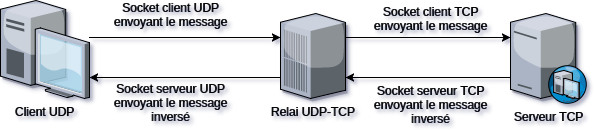
\includegraphics[width=300pt]{./cpp/Pictures/tp7+tp8-relay-UDP-TCP}
\caption{Relai UDP-TCP}
\label{Relai UDP-TCP}
\end{figure}

\inputminted[linenos,firstline=65, lastline=98]{cpp}{../sources/cpp/TP7-8/serveurTCP.c}

\section{Exercices bonus}

\subsection{Exercice 7 : Résolution de noms}
\textit{Cet exercice à pour objectif de manipuler la fonction \mintinline{cpp}{gethostbyname()}. Cette fonction permet de transformer des noms de domaines en adresse ip, en interrogeant un serveur DNS.}

\begin{figure}[H]
\centering
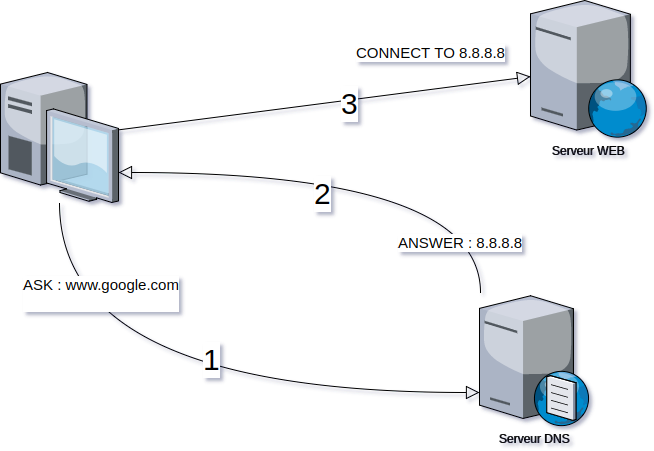
\includegraphics[width=300pt]{./cpp/Pictures/tp7+tp8-DNS}
\caption{Résolution DNS}
\label{Résolution DNS}
\end{figure}

A l’aide du manuel et des exemples disponibles sur internet, ainsi que de la documentation de la fonction \mintinline{cpp}{gethostbyname()} permettant la translation d’un nom de domaine vers une adresse IP. J'ai créé un programme qui affiche les adresses IP des noms de domaine "www.yahoo.fr", "www.gmail.com" et "www.u-bourgogne.fr".

\inputminted[linenos,firstline=10, lastline=36]{cpp}{../sources/cpp/TP7-8/getHostByName.c}

%\subsection{Exercice 8 : Serveur multi-client en mode connecté}
